\documentclass[UTF8,a4paper,11pt]{article}
\usepackage{ctex}

\usepackage{mathtools}
\usepackage{amsmath}
\usepackage{amsfonts}
\usepackage{amssymb}
\usepackage{amsthm}
\usepackage[T1]{fontenc}
\usepackage{indentfirst}

\usepackage{graphicx}
\usepackage{geometry}
\usepackage{latexsym}
\usepackage{fancyhdr}
\usepackage{titlesec}
\usepackage{setspace}
\usepackage{enumerate}
\usepackage{enumitem}
\usepackage{multicol}
\usepackage{url}
\usepackage{ulem}
\usepackage{bm}
\usepackage{hyperref}
\usepackage{stfloats}
\usepackage{listings}
\usepackage{xcolor}
\usepackage{algorithm}
\usepackage{algorithmicx}
\usepackage{algpseudocode}
\usepackage{mdframed}
\usepackage{booktabs}
\usepackage{multirow}
\usepackage{float}
\usepackage{makecell}

\setlength{\parindent}{2em}
\linespread{1.2}
\everymath{\displaystyle}
\geometry{left=2cm,right=2cm,top=2cm,bottom=2cm}
\setlength{\headheight}{14pt}
\graphicspath{{./}}
\hypersetup{hidelinks}

\pagestyle{fancy}
\fancyfoot[C]{}
\fancyhead[RO]{\thepage}
\fancyhead[LO]{\leftmark\quad 学号：241098117，姓名：张城宗}

\titleformat{\section}{\bfseries\Large}{$\S$\,\thesection\,}{1em}{}
\setenumerate[1]{itemsep=0pt,partopsep=0pt,parsep=\parskip,topsep=0pt}
\setitemize[1]{itemsep=0pt,partopsep=0pt,parsep=\parskip,topsep=0pt}

\lstdefinestyle{matlab}{
    language=Matlab,
    numbers=left,
    numberstyle=\tiny\color{gray},
    keywordstyle=\color{blue!80!black},
    commentstyle=\color{green!50!black},
    stringstyle=\color{orange!80!black},
    basicstyle=\ttfamily\small,
    frame=shadowbox,
    xleftmargin=2em,
    xrightmargin=1em,
    aboveskip=1em,
    framexleftmargin=2em,
    breaklines=true,
    showstringspaces=false,
    extendedchars=false
}

\begin{document}

\begin{center}
{\huge \textbf{数值分析第三周上机作业}}

\vspace{0.3cm}
{\large 学号：241098117\quad 姓名：张城宗\quad}
\end{center}

\section[题目一]{题目一：\texorpdfstring{$f(x)=e^x$}{f(x)=e\^x}在\texorpdfstring{$[0,1]$}{[0,1]}上的最佳平方逼近}

\subsection{问题}

求函数 $f(x)=e^x$ 在区间 $[0,1]$ 上的 $n$ 次最佳平方逼近多项式，分别考察以下四种情形：
\begin{enumerate}
  \item $n=5$，基函数取 $\phi_k(x)=x^k$；
  \item $n=5$，基函数取 $\phi_k(x)=P_k(2x-1)$；
  \item $n=10$，基函数取 $\phi_k(x)=x^k$；
  \item $n=10$，基函数取 $\phi_k(x)=P_k(2x-1)$。
\end{enumerate}
要求比较不同基函数下的逼近误差和数值稳定性。

\subsection{算法思路}

根据教材第3.4节，若 $\Phi_{n+1}=\mathrm{span}\{\phi_0,\phi_1,\dots,\phi_n\}$，则最佳平方逼近函数 $\phi^\ast(x)$ 满足
\[
\|f-\phi^\ast\|_2^2=\min_{\phi\in\Phi_{n+1}}\|f-\phi\|_2^2.
\]
令
\[
\phi(x)=\sum_{i=0}^{n} c_i\phi_i(x),
\]
则由极值条件可得法方程组
\[
\sum_{i=0}^{n} c_i(\phi_i,\phi_j)=(f,\phi_j),\qquad j=0,1,\dots,n,
\]
其中
\[
(u,v)=\int_0^1 u(x)v(x)\,\mathrm{d}x.
\]

当取幂函数基 $\phi_k(x)=x^k$ 时，
\[
G_{ij}=(x^i,x^j)=\int_0^1 x^{i+j}\,\mathrm{d}x=\frac{1}{i+j+1},
\]
因此 Gram 矩阵是 Hilbert 矩阵。教材指出该矩阵高阶时高度病态，所以虽然逼近空间相同，但数值求解容易放大舍入误差。

当取 Legendre 基 $\phi_k(x)=P_k(2x-1)$ 时，由于 Legendre 多项式在 $[-1,1]$ 上关于权函数 $W(x)=1$ 正交，线性映射到 $[0,1]$ 后，Gram 矩阵为对角阵。于是系数可直接由
\[
c_k=\frac{(f,\phi_k)}{(\phi_k,\phi_k)}
\]
计算，数值稳定性明显优于幂函数基。

\subsection{结果分析}

实验结果如表 \ref{tab:p1} 与图 \ref{fig:p1} 所示。

\begin{table}[H]
\centering
\caption{题目一结果对比}
\label{tab:p1}
\begin{tabular}{clccc}
\toprule
编号 & 情形 & $\mathrm{cond}(G)$ & $L^2$误差 & 最大误差 \\
\midrule
(1) & $n=5$，幂函数基 & $1.4951\times10^7$ & $6.9353\times10^{-7}$ & $2.5983\times10^{-6}$ \\
(2) & $n=5$，Legendre基 & $1$ & $6.9382\times10^{-7}$ & $2.5983\times10^{-6}$ \\
(3) & $n=10$，幂函数基 & $5.2232\times10^{14}$ & $1.5195\times10^{-10}$ & $6.7049\times10^{-10}$ \\
(4) & $n=10$，Legendre基 & $1$ & $2.1073\times10^{-8}$ & $6.0396\times10^{-14}$ \\
\bottomrule
\end{tabular}
\end{table}

\begin{figure}[H]
\centering
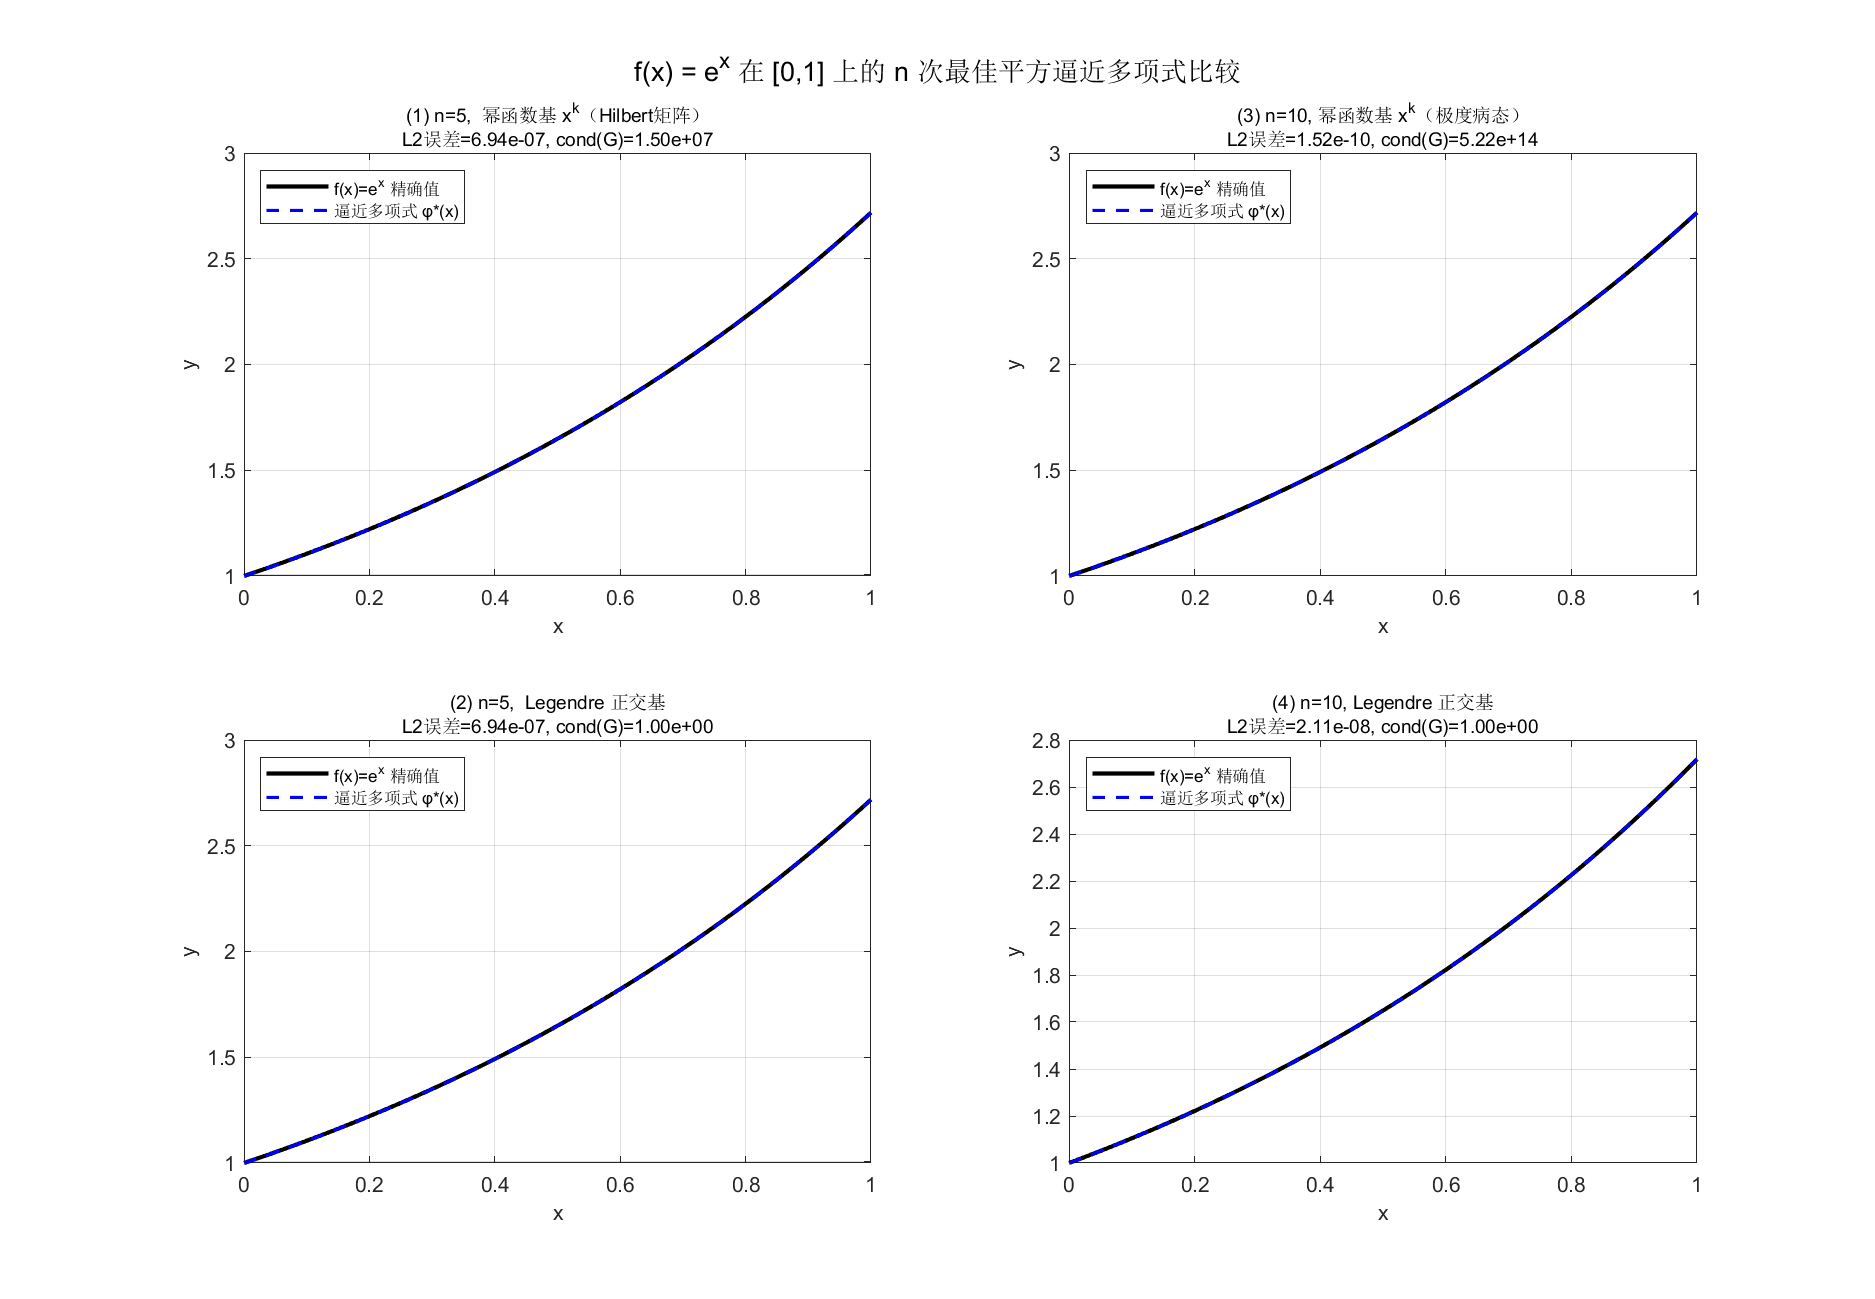
\includegraphics[width=\textwidth]{p1_fig1.png}
\caption{题目一四种最佳平方逼近结果}
\label{fig:p1}
\end{figure}

从图像上看，四条逼近曲线都与精确函数基本重合，说明在平滑函数 $e^x$ 上，多项式最佳平方逼近效果很好。但从条件数看，两类基函数差别极大。幂函数基下，Gram 矩阵条件数从 $10^7$ 迅速上升到 $10^{14}$，病态性非常明显；而 Legendre 基下条件数始终为 $1$，求解过程稳定得多。

另外，理论上不同基函数张成的是同一个多项式空间，因此最佳平方逼近结果应一致。实验中各数值略有差异，主要来自数值求解法方程时的舍入误差，而不是逼近理论本身的差异。

\subsection{结论}

本题说明：在相同的逼近空间中，\textbf{基函数的选取直接影响数值稳定性}。幂函数基虽然形式简单，但对应 Hilbert 矩阵，病态性强；Legendre 正交基可以把 Gram 矩阵化为对角阵，明显提高求解稳定性。因此在实际计算中，应优先选用正交基来构造最佳平方逼近。

\section[题目二]{题目二：例3.5.3数据的最小二乘拟合}

\subsection{问题}

利用教材例3.5.3中的10组数据
\[
\begin{aligned}
x=&(0.000,0.895,1.641,2.512,3.542,4.054,4.602,5.063,5.354,5.617),\\
y=&(1.000,1.803,3.680,7.320,13.59,17.41,22.19,24.89,26.55,29.77),
\end{aligned}
\]
完成以下两部分实验：
\begin{enumerate}
  \item 在多项式空间 $P_n$ 中做最小二乘拟合，取 $n=1,2,3,4$；
  \item 将基函数改为 $\{1,x,\cos x,\sin x\}$，比较拟合效果。
\end{enumerate}

\subsection{算法思路}

教材第3.5.1节指出，线性最小二乘拟合可转化为误差函数
\[
L(c)=\frac{1}{m}\sum_{i=1}^{m}\bigl(\phi(x_i)-y_i\bigr)^2
\]
的极小化问题。若
\[
\phi(x)=\sum_{k=0}^{n} c_k\phi_k(x),
\]
构造设计矩阵
\[
A_{ik}=\phi_{k-1}(x_i),
\]
则法方程组为
\[
(A^\mathrm{T}A)c=A^\mathrm{T}y.
\]

对于多项式拟合，设计矩阵是 Vandermonde 型矩阵，次数越高，矩阵条件数通常越大。对于一般基函数组 $\{1,x,\cos x,\sin x\}$，只要在数据点上满足 Haar 条件，最小二乘解依然唯一存在。本题程序直接使用 MATLAB 的左除运算符 \texttt{A\textbackslash y} 求解，它内部基于 QR 分解，较法方程更稳定。

\subsection{结果分析}

实验结果如表 \ref{tab:p2} 与图 \ref{fig:p2a}、图 \ref{fig:p2b} 所示。

\begin{table}[H]
\centering
\caption{题目二拟合结果对比}
\label{tab:p2}
\begin{tabular}{lccc}
\toprule
拟合方法 & $\mathrm{cond}(A)$ & RMS误差 & 均方误差 $L$ \\
\midrule
$P_1$拟合 & $8.1998\times10^0$ & $2.155425$ & $4.645856$ \\
$P_2$拟合 & $6.2211\times10^1$ & $0.553638$ & $0.306515$ \\
$P_3$拟合 & $5.4645\times10^2$ & $0.375963$ & $0.141348$ \\
$P_4$拟合 & $5.7835\times10^3$ & $0.365702$ & $0.133738$ \\
混合基拟合 & $1.3830\times10^1$ & $0.529299$ & $0.280158$ \\
\bottomrule
\end{tabular}
\end{table}

\begin{figure}[H]
\centering
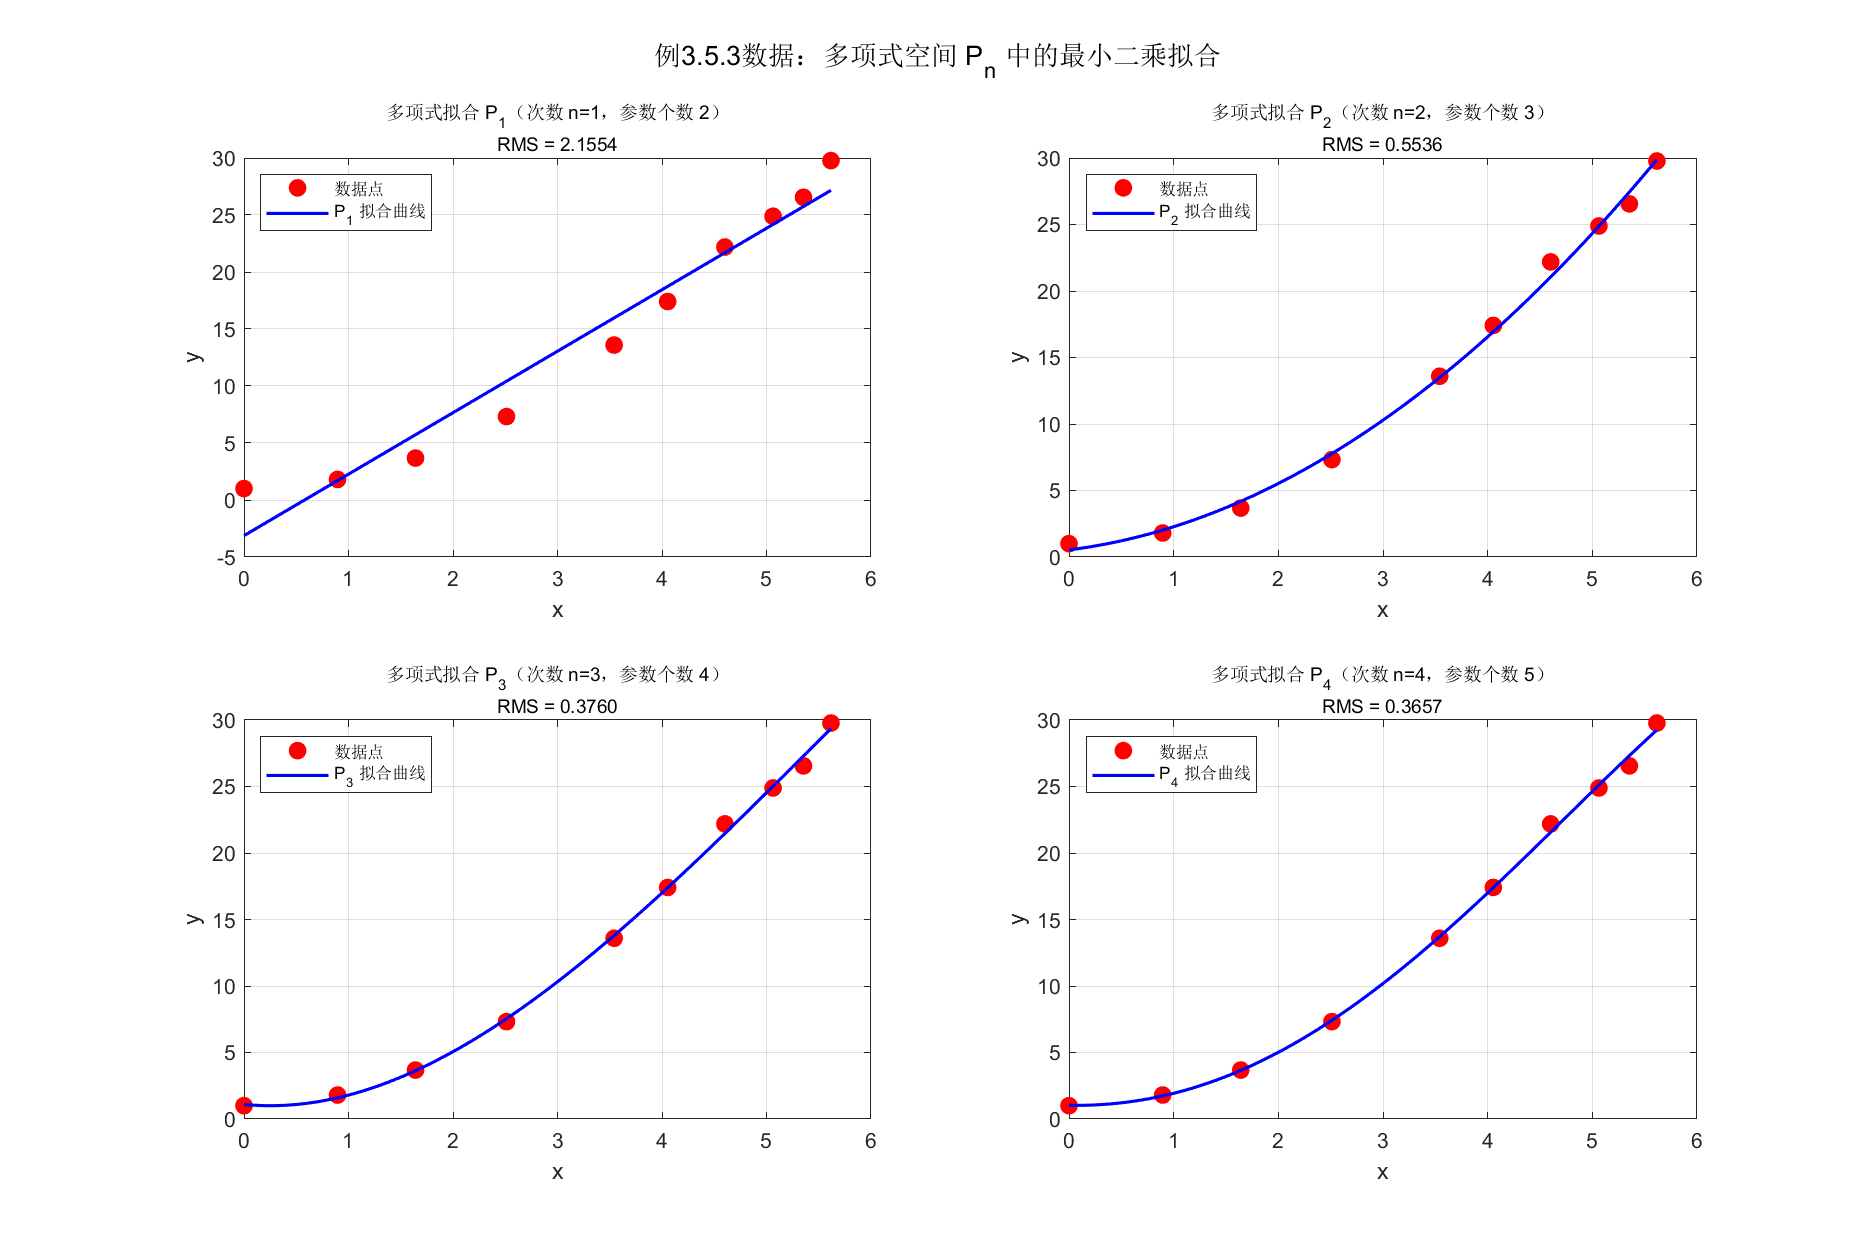
\includegraphics[width=\textwidth]{p2_fig1.png}
\caption{题目二中多项式空间 $P_n$ 的拟合结果}
\label{fig:p2a}
\end{figure}

\begin{figure}[H]
\centering
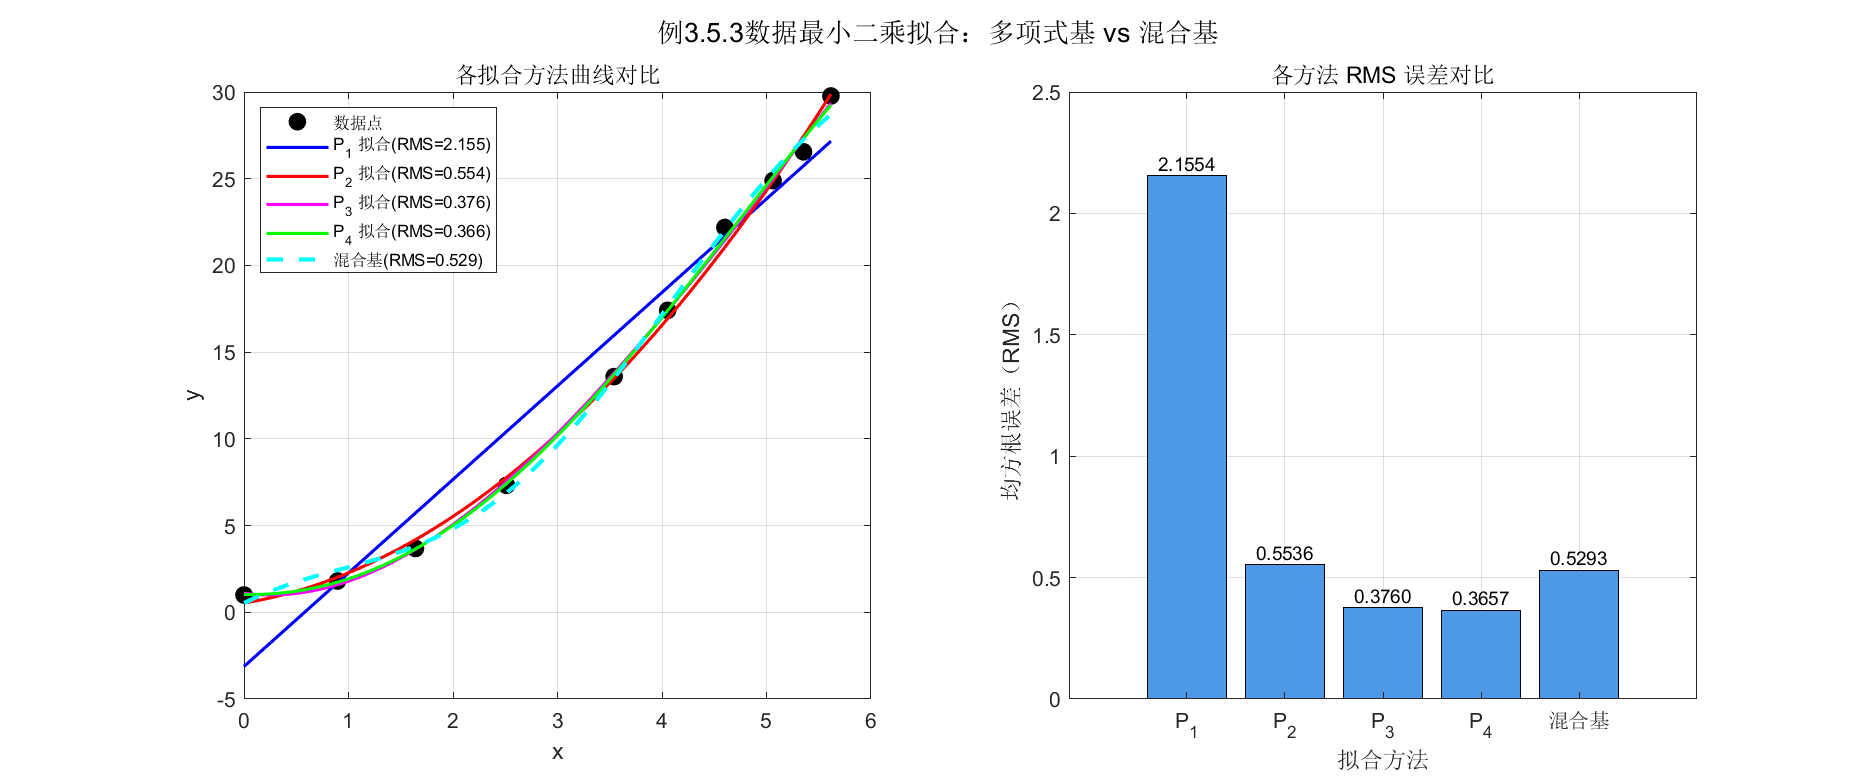
\includegraphics[width=\textwidth]{p2_fig2.png}
\caption{题目二中各方法曲线与 RMS 误差比较}
\label{fig:p2b}
\end{figure}

从结果看，随着多项式次数从 $1$ 次提高到 $4$ 次，拟合误差明显下降，说明高阶多项式对数据整体趋势的刻画更充分。但与此同时，条件数也从 $10^0$ 增长到 $10^3$ 量级，说明模型越复杂，数值稳定性越差。

混合基 $\{1,x,\cos x,\sin x\}$ 的 RMS 误差为 $0.529299$，优于一次拟合，也略优于二次拟合，但不如三次和四次多项式。这说明加入三角项后模型表达能力增强，但对这组单调上升的数据来说，多项式高次项的效果仍更好。

\subsection{结论}

本题说明最小二乘拟合需要同时考虑\textbf{精度和稳定性}。提高多项式次数确实可以减小残差，但也会增大条件数。对本题数据而言，四次多项式拟合效果最好；若兼顾模型复杂度和稳定性，则三次多项式或混合基拟合也具有一定合理性。

\section[题目三]{题目三：9次多项式拟合与条件数分析}

\subsection{问题}

仍采用例3.5.3的10组数据，令多项式次数 $n=9$，此时参数个数 $n+1=10$ 恰与数据点个数相同。要求：
\begin{enumerate}
  \item 计算幂函数基下9次多项式拟合的条件数和均方误差；
  \item 解释理论上 RMS 应为0，而计算结果却不是0的原因；
  \item 将基函数改为 Chebyshev 多项式基，比较条件数和误差变化。
\end{enumerate}

\subsection{算法思路}

当 $m=n+1$ 时，最小二乘问题退化为方阵线性系统求解问题。若数据点互不相同，则 Vandermonde 矩阵可逆，因此9次多项式拟合实际上等价于9次 Lagrange 插值。理论上应有
\[
\phi^\ast(x_i)=y_i,\qquad i=1,2,\dots,10,
\]
故残差应为零，RMS 也应为零。

但幂函数基产生的 Vandermonde 矩阵高度病态，小的舍入误差会被条件数放大，因此实际计算会出现非零残差。为改善这一问题，本题引入 Chebyshev 多项式基
\[
T_k(t)=\cos(k\arccos t),\qquad t\in[-1,1],
\]
并将原区间线性映射到 $[-1,1]$。由于 Chebyshev 基更接近正交结构，设计矩阵条件数会显著降低。

\subsection{结果分析}

结果如表 \ref{tab:p3} 与图 \ref{fig:p3} 所示。

\begin{table}[H]
\centering
\caption{题目三两种基函数的比较}
\label{tab:p3}
\begin{tabular}{lccc}
\toprule
基函数 & $\mathrm{cond}(A)$ & $\mathrm{cond}(A^\mathrm{T}A)$ & RMS误差 \\
\midrule
幂函数基 $\{x^k\}$ & $2.983236\times10^{10}$ & $3.419494\times10^{20}$ & $8.4409\times10^{-11}$ \\
Chebyshev基 $\{T_k(t)\}$ & $1.072485\times10^2$ & $1.150225\times10^4$ & $4.6428\times10^{-15}$ \\
\bottomrule
\end{tabular}
\end{table}

\begin{figure}[H]
\centering
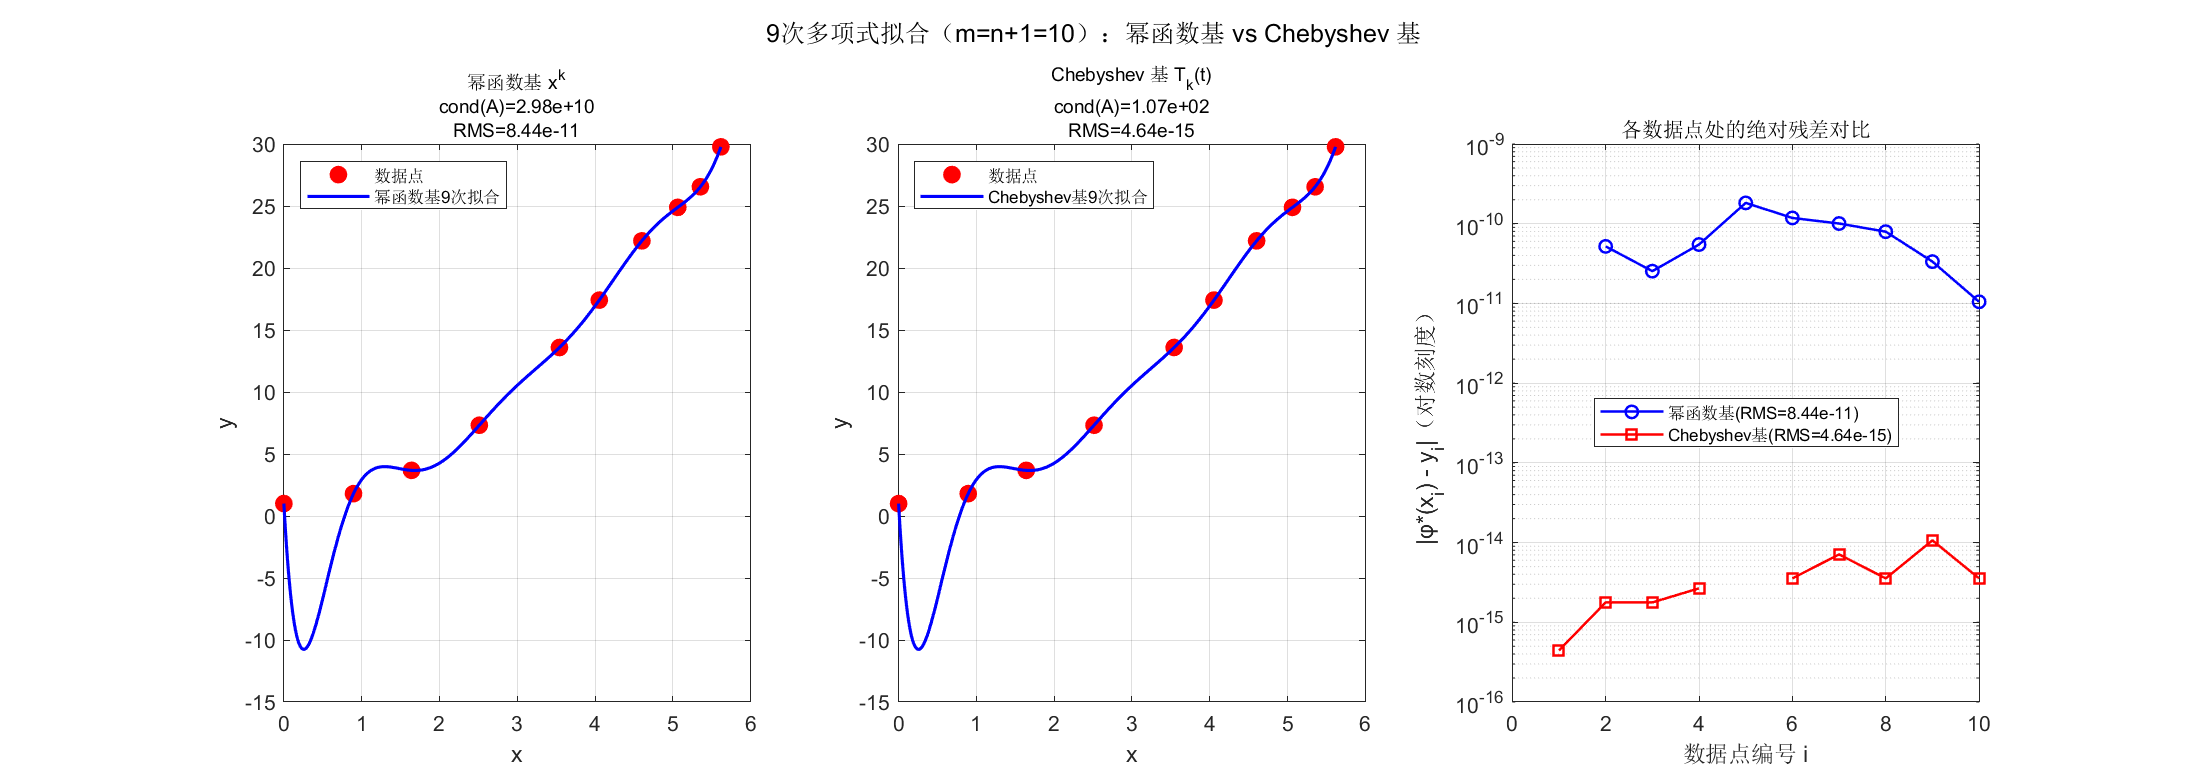
\includegraphics[width=\textwidth]{p3_fig1.png}
\caption{题目三中幂函数基与 Chebyshev 基的比较}
\label{fig:p3}
\end{figure}

由图表可以看出，两种基函数下的拟合曲线都几乎通过全部数据点，这与“$m=n+1$ 时等价于插值”的理论结论一致。但从数值层面看，幂函数基下的条件数高达 $10^{10}$ 量级，法方程矩阵更达到 $10^{20}$ 量级，是严重病态问题，因此计算得到的 RMS 仅能接近0，而不能真正等于0。

改用 Chebyshev 基后，设计矩阵条件数降低到 $10^2$ 量级，RMS 下降到 $10^{-15}$ 量级，几乎达到机器精度。这说明非零残差的根本原因不是模型错误，而是幂函数基下矩阵病态导致舍入误差被放大。

\subsection{结论}

本题表明：\textbf{理论上成立的精确插值，在数值计算中仍可能因病态矩阵而出现明显误差}。改变基函数是改善稳定性的有效手段。与幂函数基相比，Chebyshev 基显著降低了条件数，使拟合结果更接近理论零误差。

\section[题目四]{题目四：FFT算法实现与信号压缩}

\subsection{问题}

本题包括三个部分：
\begin{enumerate}
  \item 自行实现 Cooley--Tukey 基-2 FFT 算法，并与 MATLAB 内置 \texttt{fft} 对比；
  \item 利用 FFT 对合成音频信号进行频域压缩；
  \item 利用二维 FFT 对合成图像进行压缩。
\end{enumerate}

\subsection{算法思路}

教材第3.5.2节给出离散 Fourier 变换
\[
X[k]=\sum_{n=0}^{N-1}x[n]e^{-2\pi i kn/N},\qquad k=0,1,\dots,N-1,
\]
及其逆变换
\[
x[n]=\frac{1}{N}\sum_{k=0}^{N-1}X[k]e^{2\pi i kn/N}.
\]
若直接按定义计算全部频域系数，复杂度为 $O(N^2)$。FFT 的核心思想是把 $N$ 点 DFT 分解为两个 $N/2$ 点 DFT，即
\[
\begin{aligned}
X[k] &= E[k]+W_N^kO[k],\\
X[k+N/2] &= E[k]-W_N^kO[k],\qquad k=0,1,\dots,N/2-1,
\end{aligned}
\]
其中 $W_N^k=e^{-2\pi i k/N}$。这样总复杂度可降为 $O(N\log_2N)$。

在压缩应用中，若信号能量集中在少数频率分量，只保留幅值最大的若干 Fourier 系数，再用逆 FFT 重建，就能实现有损压缩。保留比例越高，重建越接近原信号；保留比例越低，压缩率更高，但失真也更明显。

\subsection{结果分析}

\textbf{1. FFT正确性验证}：对长度 $N=64$ 的复数测试信号，自实现 FFT 与 MATLAB 内置 \texttt{fft} 的最大误差为
\[
1.0658\times10^{-14},
\]
说明算法实现正确。

\textbf{2. 音频信号压缩}：主要频率分量和压缩结果见表 \ref{tab:p4a}、表 \ref{tab:p4b}，图 \ref{fig:p4a} 给出了重建效果。

\begin{table}[H]
\centering
\caption{题目四音频信号主要频率分量}
\label{tab:p4a}
\begin{tabular}{ccc}
\toprule
序号 & 频率(Hz) & 幅度 \\
\midrule
1 & 49.80 & 941.20 \\
2 & 120.12 & 484.57 \\
3 & 50.78 & 246.34 \\
4 & 200.20 & 237.16 \\
5 & 48.83 & 151.66 \\
\bottomrule
\end{tabular}
\end{table}

\begin{table}[H]
\centering
\caption{题目四音频信号压缩结果}
\label{tab:p4b}
\begin{tabular}{cccc}
\toprule
保留比例 & 系数个数 $K$ & RMS误差 & SNR \\
\midrule
$20\%$ & 205 & 0.1641 & 19.9 dB \\
$5\%$ & 51 & 0.2273 & 17.1 dB \\
$1\%$ & 10 & 0.3903 & 12.4 dB \\
\bottomrule
\end{tabular}
\end{table}

\begin{figure}[H]
\centering
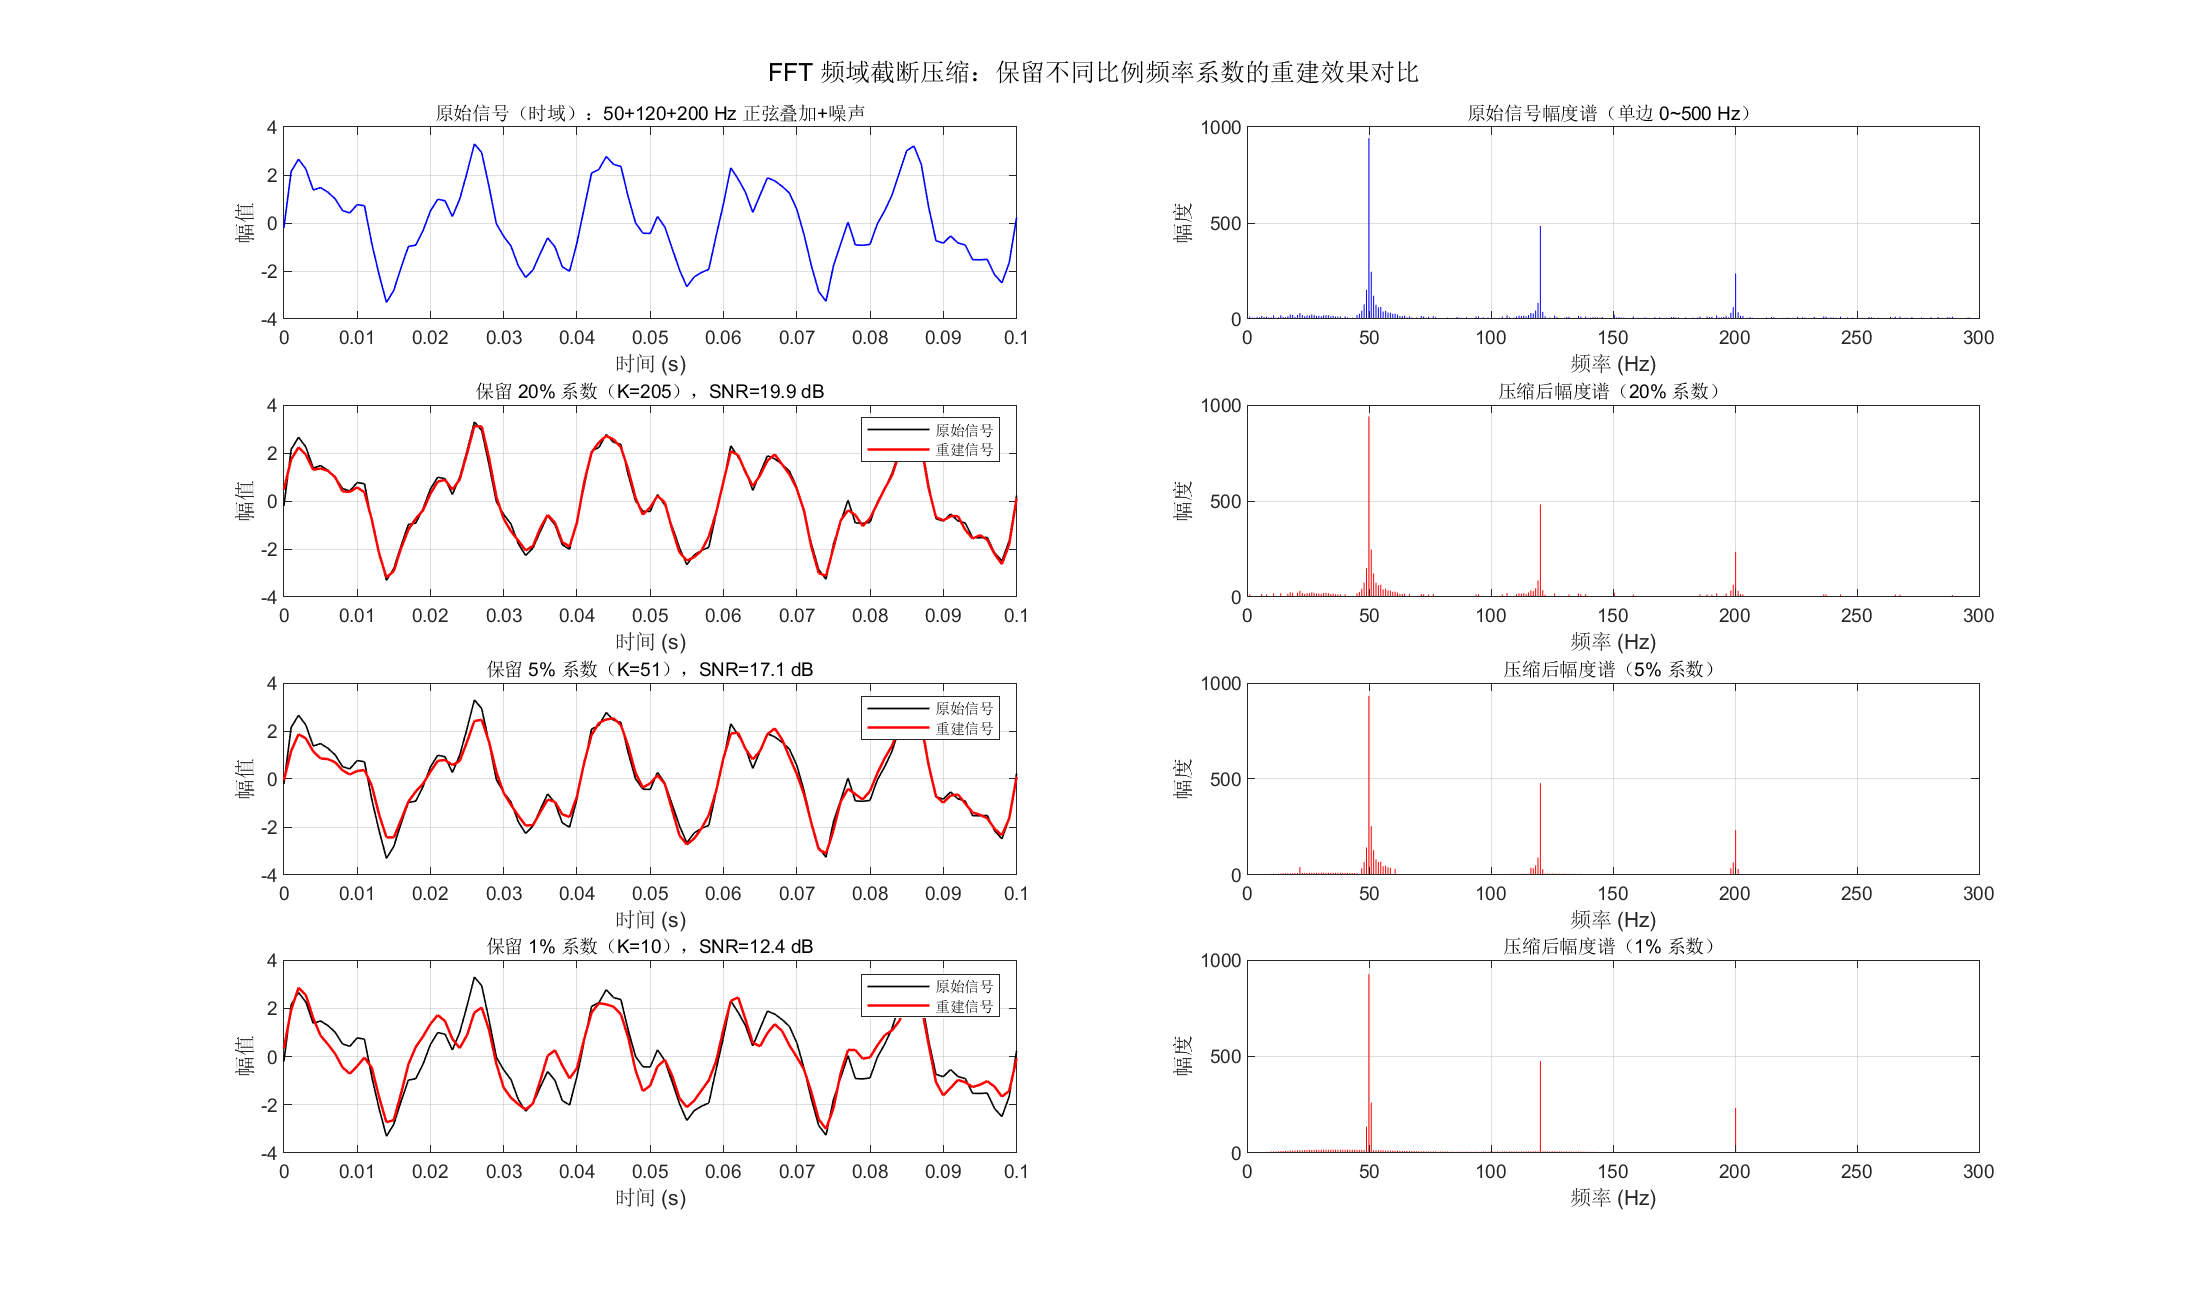
\includegraphics[width=\textwidth]{p4_fig1.png}
\caption{题目四音频信号在不同比例频域截断下的重建效果}
\label{fig:p4a}
\end{figure}

从图像可以看出，保留 $20\%$ 系数时重建波形与原信号较接近；保留 $5\%$ 时主频结构仍在，但细节开始损失；仅保留 $1\%$ 时失真已经比较明显。这说明该信号的大部分能量集中在少数频率成分上，FFT 压缩是有效的。

\textbf{3. 图像压缩}：结果如表 \ref{tab:p4c} 与图 \ref{fig:p4b} 所示。

\begin{table}[H]
\centering
\caption{题目四图像压缩结果}
\label{tab:p4c}
\begin{tabular}{ccc}
\toprule
保留比例 & 保留系数个数 & 图像SNR \\
\midrule
$10\%$ & 410 & 24.6 dB \\
$2\%$ & 82 & 23.3 dB \\
\bottomrule
\end{tabular}
\end{table}

\begin{figure}[H]
\centering
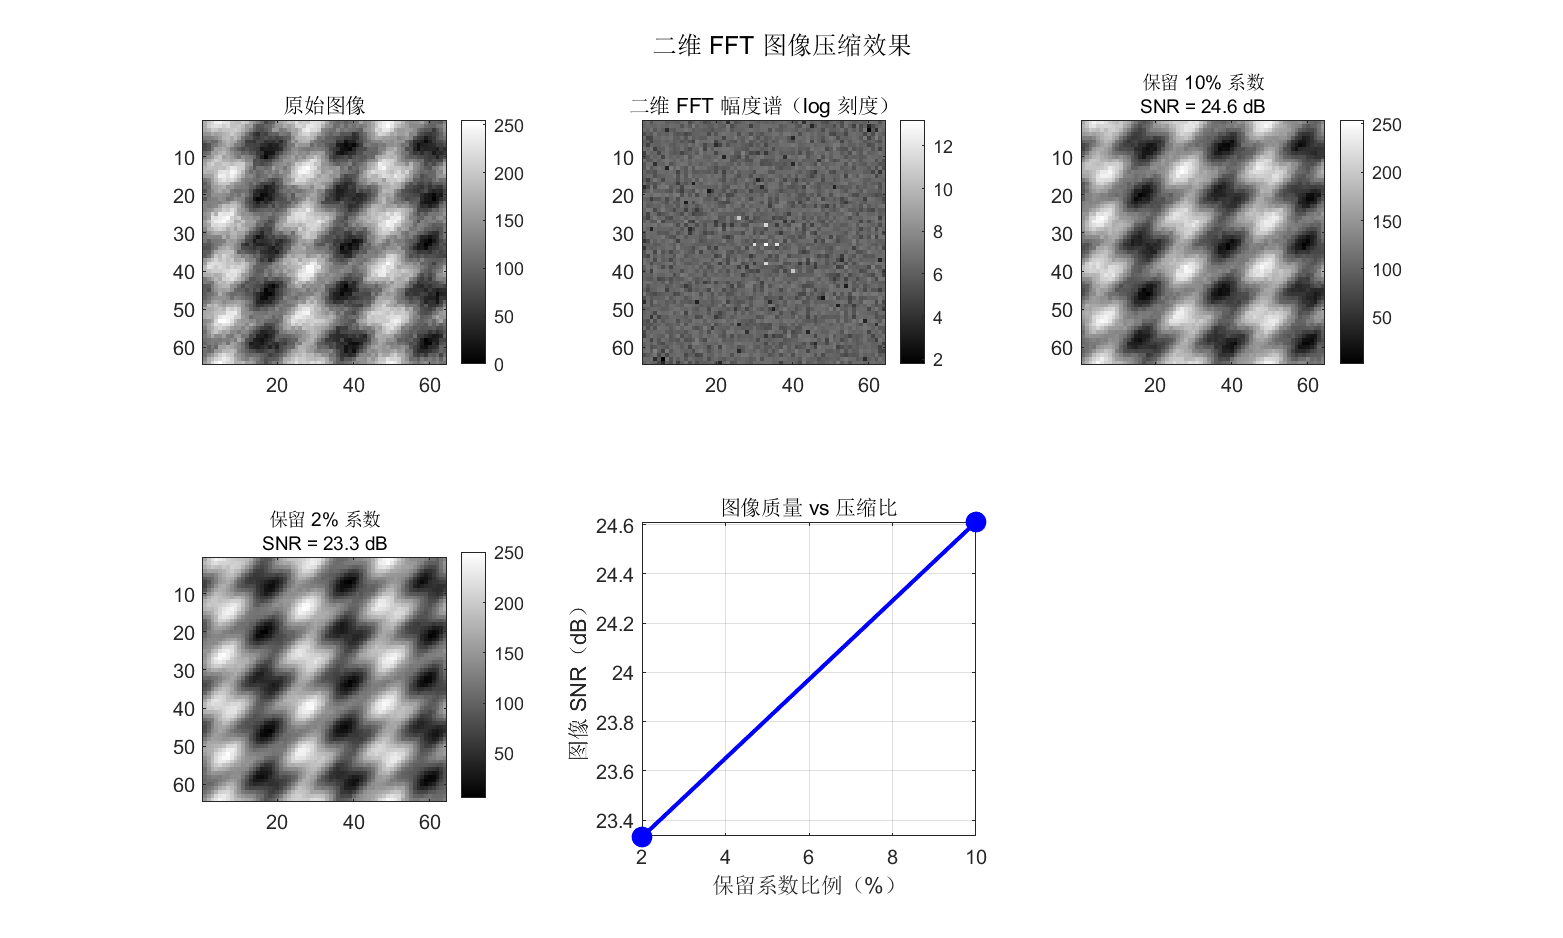
\includegraphics[width=\textwidth]{p4_fig2.png}
\caption{题目四二维FFT图像压缩效果}
\label{fig:p4b}
\end{figure}

二维频谱图显示，图像能量集中在少数低频和特征频率附近。即使只保留 $2\%$ 的频率系数，图像整体纹理仍然较清晰；保留 $10\%$ 时图像更接近原图，SNR 也更高。

\subsection{结论}

本题说明 FFT 不仅在理论上能把 DFT 的复杂度由 $O(N^2)$ 降到 $O(N\log N)$，而且在实际应用中也是高效的频域分析与压缩工具。无论是一维音频信号还是二维图像，只要频谱能量具有集中性，就可以通过保留主要频率系数实现较好的压缩效果。

\clearpage

\section[附录]{附录：程序代码}

\subsection{题目一关键代码}

\begin{lstlisting}[style=matlab, caption={最佳平方逼近中幂函数基与Legendre基的核心实现}]
f = @(x) exp(x);
f_L2sq = (exp(2) - 1) / 2;
x_plot = linspace(0, 1, 500);
y_exact = f(x_plot);

for n = [5, 10]
    G = hilb(n + 1);
    f_vec = zeros(n + 1, 1);
    for j = 0:n
        f_vec(j + 1) = integral(@(x) exp(x) .* x.^j, 0, 1);
    end
    c_mono = G \ f_vec;
    kappa_G = cond(G);

    phi_mono = zeros(size(x_plot));
    for k = 0:n
        phi_mono = phi_mono + c_mono(k + 1) * x_plot.^k;
    end
    L2_err_mono = sqrt(integral(@(x) (exp(x) - polyval(flipud(c_mono), x)).^2, 0, 1));

    c_leg = zeros(n + 1, 1);
    for k = 0:n
        inner_fk = integral(@(x) exp(x) .* legendre_on_01(k, x), 0, 1);
        c_leg(k + 1) = (2 * k + 1) * inner_fk;
    end
    phi_leg = zeros(size(x_plot));
    for k = 0:n
        phi_leg = phi_leg + c_leg(k + 1) * legendre_on_01(k, x_plot);
    end
    max_err_leg = max(abs(y_exact - phi_leg));
end
\end{lstlisting}

算例结果：$n=10$ 时，幂函数基对应 $\mathrm{cond}(G)=5.2232\times10^{14}$，而 Legendre 基对应 $\mathrm{cond}(G)=1$。

\subsection{题目二关键代码}

\begin{lstlisting}[style=matlab, caption={最小二乘拟合的设计矩阵构造、求解与误差计算}]
x_data = [0.000, 0.895, 1.641, 2.512, 3.542, 4.054, 4.602, 5.063, 5.354, 5.617];
y_data = [1.000, 1.803, 3.680, 7.320, 13.59, 17.41, 22.19, 24.89, 26.55, 29.77];
x_plot = linspace(min(x_data), max(x_data), 500);

for n = [1, 2, 3, 4]
    A = zeros(length(x_data), n + 1);
    for k = 0:n
        A(:, k + 1) = x_data(:).^k;
    end
    c = A \ y_data(:);
    y_fit = A * c;
    rms_err = sqrt(mean((y_fit - y_data(:)).^2));
    kappa_A = cond(A);

    A_plot = zeros(length(x_plot), n + 1);
    for k = 0:n
        A_plot(:, k + 1) = x_plot(:).^k;
    end
    fit_poly = A_plot * c;
end

A_mix = [ones(length(x_data), 1), x_data(:), cos(x_data(:)), sin(x_data(:))];
c_mix = A_mix \ y_data(:);
y_fit_mix = A_mix * c_mix;
rms_mix = sqrt(mean((y_fit_mix - y_data(:)).^2));
\end{lstlisting}

算例结果：四次多项式拟合的 RMS 误差为 $0.365702$，混合基拟合的 RMS 误差为 $0.529299$。

\subsection{题目三关键代码}

\begin{lstlisting}[style=matlab, caption={9次多项式拟合中Chebyshev基与幂函数基的对比实现}]
m = length(x_data);
n = m - 1;

A_mono = zeros(m, n + 1);
for k = 0:n
    A_mono(:, k + 1) = x_data(:).^k;
end

a = min(x_data);
b = max(x_data);
t_data = (2 * x_data - (a + b)) / (b - a);

A_cheby = zeros(m, n + 1);
for k = 0:n
    A_cheby(:, k + 1) = cos(k * acos(t_data(:)));
end

c_mono = A_mono \ y_data(:);
c_cheby = A_cheby \ y_data(:);
kappa_mono = cond(A_mono);
kappa_cheby = cond(A_cheby);

y_fit_mono = A_mono * c_mono;
y_fit_cheby = A_cheby * c_cheby;
rms_mono = sqrt(mean((y_fit_mono - y_data(:)).^2));
rms_cheby = sqrt(mean((y_fit_cheby - y_data(:)).^2));
\end{lstlisting}

算例结果：幂函数基下 $\mathrm{cond}(A)=2.983236\times10^{10}$，Chebyshev 基下 $\mathrm{cond}(A)=1.072485\times10^2$。

\subsection{题目四关键代码}

\begin{lstlisting}[style=matlab, caption={基-2 FFT递归实现与频域压缩核心代码}]
function X = my_fft(x)
    N = length(x);
    if N == 1
        X = x;
        return;
    end
    x_even = x(1:2:end);
    x_odd  = x(2:2:end);
    E = my_fft(x_even);
    O = my_fft(x_odd);
    k = 0 : N / 2 - 1;
    W = exp(-2i * pi * k / N);
    X = [E + W .* O, E - W .* O];
end

Fs = 1000;
t = 0 : 1 / Fs : 1 - 1 / Fs;
x_signal = 2.0 * sin(2 * pi * 50 * t) ...
         + 1.0 * sin(2 * pi * 120 * t) ...
         + 0.5 * sin(2 * pi * 200 * t) ...
         + 0.2 * randn(size(t));

N_sig = length(t);
N_fft = 2^nextpow2(N_sig);
x_padded = [x_signal, zeros(1, N_fft - N_sig)];
X_freq = my_fft(x_padded);

ratio = 0.20;
K = round(ratio * N_fft);
[~, idx_sorted] = sort(abs(X_freq), 'descend');
X_compressed = zeros(size(X_freq));
X_compressed(idx_sorted(1:K)) = X_freq(idx_sorted(1:K));

x_rec = real(my_ifft(X_compressed));
x_rec = x_rec(1:N_sig);
rms_err = sqrt(mean((x_rec - x_signal).^2));
snr_db = 20 * log10(norm(x_signal) / norm(x_rec - x_signal));
\end{lstlisting}

算例结果：自实现 FFT 与 MATLAB 内置 \texttt{fft} 的最大误差为 $1.0658\times10^{-14}$；音频信号保留 $20\%$ 频率系数时，SNR 为 $19.9\,\mathrm{dB}$。

\end{document}
